\documentclass[journal]{IEEEtran}
\usepackage[T1]{fontenc}
\usepackage{amsmath,amssymb}
\usepackage{graphicx}
\usepackage{booktabs}
\usepackage{cite}
\usepackage{xcolor}
\usepackage{url}
\usepackage[font=small,labelfont=bf,labelsep=period]{caption}
\usepackage{balance}
\usepackage[hidelinks]{hyperref}
\hypersetup{pdftitle={AxisCodec: Geometry-Aware CSI Feedback on the Angular-Delay Cylinder},
  pdfauthor={Ziheng Wang and Kimi Code},
  pdfkeywords={CSI feedback, massive MIMO, angular-delay, physics-informed learning}}

\graphicspath{{figures/}}
\setlength{\emergencystretch}{1.2em}

\newcommand{\Hb}{\mathbf{H}}
\newcommand{\Hh}{\hat{\mathbf{H}}}
\newcommand{\Cx}{\mathbb{C}}
\newcommand{\R}{\mathbb{R}}
\newcommand{\dd}{\mathrm{d}}

\begin{document}

\title{AxisCodec: Geometry-Aware CSI Feedback\\on the Angular--Delay Cylinder}

\author{Ziheng Wang and Kimi Code%
\thanks{Z. Wang: \texttt{666zihengwang@gmail.com}. Manuscript prepared November
2026. Code, configurations and metric records are available in the accompanying
repository.}}

\markboth{IEEE Transactions on Wireless Communications (submitted)}%
{AxisCodec: Geometry-Aware CSI Feedback}

\maketitle

\begin{abstract}
Deep-learning CSI feedback compresses the angular--delay channel as if it were an
image. A recent line of work goes further and treats the image as a handful of
propagation paths, transmitting their angles, delays and gains. We test that
assumption on COST2100 with rate-matched oracle experiments and find that it fails:
four Dirichlet atoms explain only $-5.2$~dB where a free-support sparse code of the
same size reaches $-8.0$~dB, and none of our parametric fits exceeds $-5.2$~dB at
any budget we tried, while the sparse code reaches $-21.0$~dB with 128 complex
coefficients. The energy is diffuse
(99\% of it needs about 105 complex coefficients), and the residual of the strongest
baseline concentrates in the delay tail, which cannot be extrapolated from the head.
Guided by these measurements we build AxisCodec around the geometry of the
\emph{representation} rather than a parametric channel model: the angle axis is a
circle and the delay axis is a half-line, so angle mixing is a circulant operator
(32 parameters per channel) and delay mixing is a dense $32\times32$ map. A linear
base plus a nonlinear residual decoder, trained with the per-user NMSE that the
benchmark actually reports, reaches $-32.52\pm0.55$~dB at CR~$1/4$ against
$-30.17$~dB for STNet, with the same effective parameter count and $1.6\times$
its FLOPs.
\end{abstract}

\begin{IEEEkeywords}
CSI feedback, massive MIMO, angular--delay domain, physics-informed learning,
rate--distortion.
\end{IEEEkeywords}

\section{Introduction}
\IEEEPARstart{F}{requency-division} duplex massive MIMO needs the user equipment to
report downlink channel state information (CSI) over a narrow uplink control
channel. The dominant recipe first applies a two-dimensional DFT to the
space--frequency channel and keeps the first 32 delay taps, producing a
$32\times32$ angular--delay image with real and imaginary parts as two channels
\cite{wen2018}. CsiNet then compresses this image with a convolutional encoder, a
fully connected bottleneck and a refinement decoder \cite{wen2018}. Later work
enlarged the receptive field with multi-resolution convolutions \cite{lu2020},
switched to complex-valued and lightweight designs \cite{ji2021,cvl2022}, and added
attention: full attention \cite{cui2022}, spatially separable attention
\cite{mourya2023}, and hybrids with CNN stems \cite{lou2025,ansarifard2025}.

A parallel line replaces the image codec by a parametric one: estimate a few
propagation paths, transmit their angles, delays and gains, and synthesise the
channel at the receiver \cite{guo2022model,liu2022markov,ma2023typeii}. The appeal
is obvious: a far-field channel is a sum of plane waves.

This paper starts by asking whether that is true for the standard benchmark. We answer with rate-matched oracle fits rather than with another architecture.
On COST2100 indoor, an oracle fit of $k$ continuous Dirichlet atoms, an oracle
harmonic subspace of $r$ modes with $m$ coefficients per singular vector, and an
oracle fit of $k$ two-dimensional Gaussian blobs all fall far behind a
free-support sparse code of the same size (Section~\ref{sec:where}). The angular--delay
energy is diffuse: 99\% of it requires about 105 of the 1024 complex coefficients.
The physical prior that the field is a few clean paths is simply not a property of
this data.

The measurements also say where the error \emph{does} live. For STNet
\cite{mourya2023}, the strongest baseline on this benchmark, 69\% of the residual
energy sits in delay taps 4--31, which carry only 7.9\% of the signal. A linear
predictor trained on the head explains 23\% of the tail variance, so the tail is
independent information rather than an analytic continuation. At the same time, at
CR~$1/4$ a 512-dimensional linear subspace (PCA) is already within 1~dB of STNet:
the low-rate end of the curve is nearly saturated by a linear method.

These two observations motivate a different use of physics. Instead of encoding a
parametric channel model, we encode the geometry of the \emph{representation}.
The angular--delay image lives on a half-open cylinder: the angle axis is a circle,
because the uniform linear array manifold is periodic in spatial frequency (we
measure the energy wrapping from bin 31 to bin 0), while the delay axis is a
half-line with no shift invariance (92.2\% of the energy is in the first four taps
and the profile decays monotonically). AxisCodec therefore mixes angles with a
circulant operator---a learned filter in the DFT domain, 32 parameters per
channel---and delays with a dense $32\times32$ map that gives every tap its own
read-out. The decoder splits into a linear base and a nonlinear residual, and the
training objective is the per-user normalised MSE that the benchmark reports,
with checkpoint selection moved to the validation split.

Our contributions are: (i) a rate-matched diagnostic that rules out compact
parametric channel models on COST2100 and locates the residual in the delay tail;
(ii) AxisCodec, which turns that diagnosis into a geometry-constrained codec of
matched complexity; and (iii) a controlled study showing $-32.52\pm0.55$~dB at
CR~$1/4$ versus $-30.17$~dB for STNet, gains at every measured compression ratio,
and ablations that attribute 1.50~dB to the objective, 0.44~dB to the linear base
and 0.25~dB to the circulant angle prior.

\section{Related Work}
\textbf{Autoencoder codecs.} CsiNet \cite{wen2018} established the architecture
that most later work still follows: convolutional encoder, fully connected
bottleneck, refinement decoder. CRNet added multi-resolution paths and anisotropic
$1\times9$/$9\times1$ kernels \cite{lu2020}. CsiNet-LSTM exploited temporal
correlation \cite{wang2019}. CLNet fed complex values to a lightweight network
\cite{ji2021}, and CVLNet extended the idea with complex-valued layers
\cite{cvl2022,trabelsi2018}.

\textbf{Attention.} TransNet applies full self-attention to the angular--delay
image \cite{cui2022}. STNet, our strongest baseline, alternates grouped and global
attention with convolutional refinement \cite{mourya2023}. Hybrid attention--CNN
designs and entropy-regularised variants followed \cite{lou2025,ansarifard2025},
as did attention over the recovery stage \cite{cai2019,saldr2021}.

\textbf{Model-driven and parametric priors.} Unrolled estimators replace iterative
recovery \cite{guo2022model}, Markovian priors model temporal structure
\cite{liu2022markov}, and deep Type-II codebooks learn the codebook itself
\cite{ma2023typeii,qin2025}; the standardized Type-II codebook is the reference
this family improves on \cite{3gpp38214}, and 3GPP is now studying AI/ML
compression itself \cite{3gpp38843}. EVCsiNet feeds back eigenvectors instead of
the raw matrix \cite{liu2021ev}. Our diagnostic in Section~\ref{sec:where} quantifies what
this family can and cannot buy on COST2100.

\textbf{Generative and task-oriented decoders.} Diffusion-based compression treats
low-rate recovery as an under-determined inverse problem \cite{kim2025}.
System-level views argue that NMSE is only a proxy for beamforming gain
\cite{guo2025onesided}. We keep the standard NMSE/$\rho$ protocol for comparability
and report $\rho$ separately, because it moves differently at high compression.

\section{Where the Error Lives}\label{sec:where}
\subsection{The representation is a half-open cylinder}
With half-wavelength spacing, the array response of a path at angle $\theta$ is
$a_n(\theta)=e^{j\pi n\sin\theta}$, and its $N_a$-point DFT is a Dirichlet kernel
\begin{equation}
A_i(f)=\frac{\sin(\pi(f-i))}{\sin(\pi(f-i)/N_a)}
e^{j\pi(N_a-1)(f-i)/N_a},\quad f=\tfrac12\sin\theta,
\end{equation}
with $f\in[-\tfrac12,\tfrac12)$. The angle axis is therefore a \emph{circle}: bin 0
and bin 31 are neighbouring beams. The data agrees---the mean energy rises again at
bins 30 and 31 ($2.6\%$ and $3.7\%$ of the angular profile) after decaying through
the sector (Fig.~\ref{fig:geo}b). The delay axis is the opposite: delay is
non-negative, 92.2\% of the energy sits in taps 0--3, and the profile decays by two
orders of magnitude over the next twelve taps (Fig.~\ref{fig:geo}c). There is no
shift invariance along delay.

\begin{figure*}[!t]
\centering
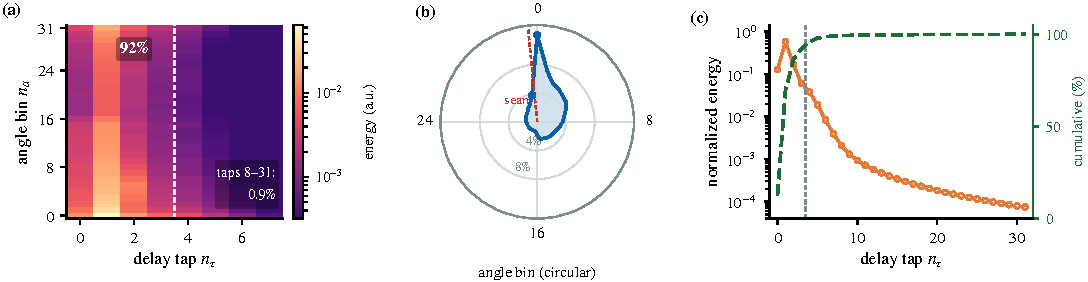
\includegraphics[width=\textwidth]{fig1_geometry.pdf}
\caption{The angular--delay representation is a half-open cylinder.
(a) Mean energy over the test set for delay taps 0--7. The colour scale saturates
below $-16$~dB; taps 8--31 hold 0.9\% of the energy. (b) Angular profile on the
circle: the energy wraps across the bin~31/bin~0 boundary. (c) Delay profile
(log scale) and its cumulative sum; the dashed line marks the 92.2\% head used
throughout the paper.}
\label{fig:geo}
\end{figure*}

\subsection{Compact propagation models do not fit}
We fit three parametric families per sample and measure the NMSE at the rate each
family would cost. \emph{Dirichlet atoms} are the separable plane-wave response of
(1): $k$ atoms with continuous angle, delay and complex gain. \emph{Harmonic
subspaces} keep the first $r$ singular modes of the sample and truncate each
singular vector to its $m$ largest DFT coefficients. \emph{Gaussian blobs} are $k$
separable two-dimensional Gaussian envelopes with spreads.

Table~\ref{tab:oracle} collects the results next to a free-support sparse code and
a free-basis rank-$r$ approximation. No parametric family comes close. A single
Dirichlet atom reaches $-0.34$~dB where a 16-term sparse code---eight times its
budget---reaches $-9.5$~dB; a 66-coefficient harmonic subspace reaches $-2.44$~dB,
27~dB behind a 512-dimensional PCA subspace; four blobs reach $-5.16$~dB where a
sparse code of the same size reaches $-8.0$~dB. The reason is visible in
Fig.~\ref{fig:geo}a: the energy is spread over tens of one-to-two-bin clusters,
not concentrated in a few paths. A 99\%-energy support needs about 105 complex
coefficients.

\begin{table}[!t]
\centering
\caption{Parametric oracles versus free-support sparse codes on COST2100 indoor.
NMSE in dB, lower is better. The sparse code sends the $k$ largest complex
coefficients with their positions free; $k$ is chosen so that its $2k$ real
coefficients meet or exceed the budget of the parametric model, which biases the
comparison towards the free reference.}
\label{tab:oracle}
\footnotesize
\setlength{\tabcolsep}{3.6pt}
\begin{tabular}{@{}lccccc@{}}
\toprule
Model & reals & NMSE & sparse $k$ & reals & NMSE \\
\midrule
1 Dirichlet atom & 4 & $-0.34$ & 16 & 32 & $-9.53$\\
4 Dirichlet atoms & 16 & $-5.20$ & 16 & 32 & $-9.53$\\
Harmonic $r{=}1,m{=}16$ & 66 & $-2.44$ & 32 & 64 & $-12.55$\\
4 Gaussian blobs & 24 & $-5.16$ & 12 & 24 & $-8.00$\\
PCA subspace & 512 & $-29.22$ & 256 & 512 & $-27.34$\\
\bottomrule
\end{tabular}
\end{table}

\subsection{The error is in the delay tail}
We decompose the residual of the strongest baseline, STNet at CR~$1/4$
($-30.17$~dB), over the test set. Taps 0--3 carry 92.1\% of the signal but only
31\% of the error, with a relative error of $3.7\times10^{-4}$; taps 4--31 carry
7.9\% of the signal and 69\% of the error, with a relative error of
$9.4\times10^{-3}$, thirty times worse (Fig.~\ref{fig:err}). The concentration is
structural: taps 7--9 alone account for 42\% of the total error while carrying
0.7\% of the energy, and PCA shows the same pattern even more sharply.

The tail is not predictable from the head. A ridge regressor trained on 40k
samples to map taps 0--3 to taps 4--31 explains 23\% of the tail variance, whereas
STNet already reconstructs the tail to 1\% relative error. The tail therefore has
to be transmitted; it is where the bits should go. Conversely, at CR~$1/4$ a
512-dimensional PCA subspace reaches $-29.2$~dB, within 1~dB of STNet, so the
low-rate end has little nonlinear headroom and the tail is what separates good
from mediocre codecs.

\begin{figure}[!t]
\centering
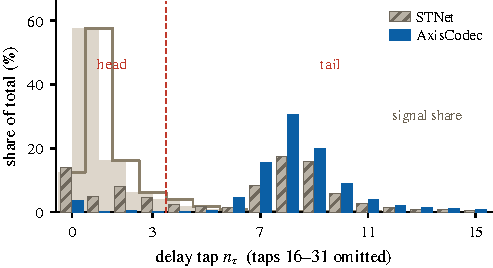
\includegraphics[width=\columnwidth]{fig2_error.pdf}
\caption{Per-tap error share at CR~$1/4$ for STNet and AxisCodec, against the
signal share (shaded). Both models push their error into taps~4--31; AxisCodec
does so with a smaller total, and its head relative error is twelve times lower.}
\label{fig:err}
\end{figure}

\section{Method}
\subsection{Geometry-correct operators}
The analysis above argues for encoding the geometry of the representation, not a
parametric channel. AxisCodec keeps the standard $2\times32\times32$ input and
replaces every spatial operator by one that respects the cylinder.

\textbf{Angle mixer.} Angles form a circle, so the natural operator is a circular
convolution. We implement it as a learned filter in the DFT domain,
\begin{equation}
\mathrm{Mix}_a(x)_c=\mathcal F^{-1}\!\Big(\mathcal F(x_c)\odot w_c\Big),\qquad
w_c\in\Cx^{17},
\end{equation}
which is exactly shift-equivariant on the circle and costs 32 real parameters per
channel instead of the $32^2$ of a dense map. The grid is preserved (no pooling),
so fine angular structure survives.

\textbf{Delay mixer.} Delay is a half-line: there is no shift invariance, and the
statistics of tap 0 differ from those of tap 20. We therefore use a dense
$32\times32$ map applied along the delay axis, shared across channels. Every tap
gets its own read-out; zero padding at the boundary reflects the absence of
negative delay.

A block applies layer normalisation, the angle mixer, a GELU, the delay mixer, a
GELU and a $1\times1$ channel MLP of twice the channel width, wrapped in a residual
connection. Eight blocks are stacked; both mixers are global along their
axis, so a single block already couples every angle bin and every delay tap.
Per-position layer normalisation keeps the weakly energetic delay tail on the same
numerical footing as the head.

\subsection{Linear base and nonlinear residual}
The decoder separates what a linear map does well from what it does not:
\begin{equation}
\Hh = \underbrace{P z}_{\text{linear base}}+\underbrace{g_\theta(z)}_{\text{residual}},
\qquad \hat x = 0.5+\Hh,
\end{equation}
with $z\in\R^{D}$, $D=2048/\mathrm{CR}$, $P\in\R^{2048\times D}$ learned, and
$g_\theta$ the block stack described above (Fig.~\ref{fig:arch}). The base carries
the bulk of the energy, which is spatially smooth, and the residual corrects it.
Section~\ref{sec:exp} shows that this split lowers the head relative error from
$3.7\times10^{-4}$ to $3.0\times10^{-5}$ and moves essentially all of the error
into the tail, where the nonlinear stack can work on it.

\begin{figure*}[!t]
\centering
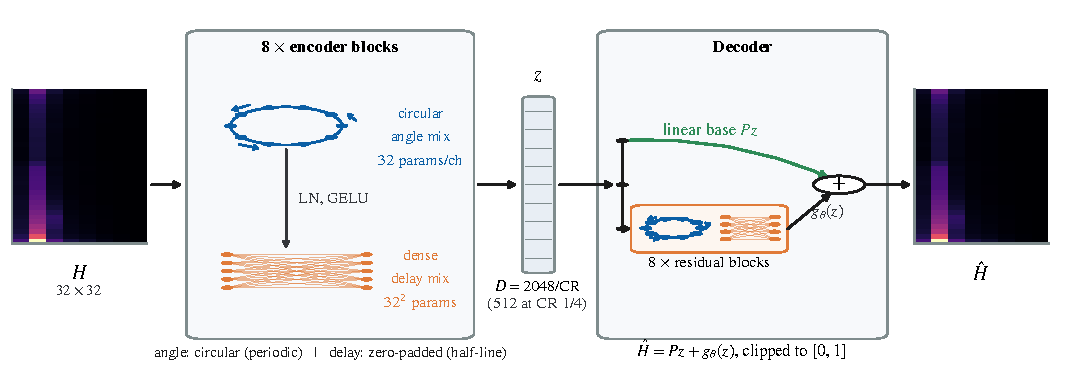
\includegraphics[width=\textwidth]{fig3_arch.pdf}
\caption{AxisCodec. The encoder alternates a circulant angle mixer
(32 parameters per channel, exact circular shift equivariance) with a dense delay
mixer ($32^2$ parameters, one read-out per tap). The decoder adds a linear base
$Pz$ and a nonlinear residual trunk before clipping to the valid CSI range.}
\label{fig:arch}
\end{figure*}

\subsection{Metric-aligned objective}
Baselines train with element-wise MSE, but the benchmark reports the per-user
normalised error
\begin{equation}
\mathrm{NMSE}=\frac{1}{B}\sum_{i=1}^{B}
\frac{\lVert\hat x_i-x_i\rVert_F^2}{\lVert x_i-0.5\rVert_F^2}.
\end{equation}
Here $x_i$ is the two-channel image and $\hat x_i$ the reconstruction (3).
The two weight samples differently: MSE weights by power, NMSE does not, and its
mean is dominated by the samples a model currently fails on. We minimise (4)
directly (without the logarithm) and---this matters for the ablation---select the
checkpoint with the same quantity on the validation split. When an ablation
replaces the training loss by MSE, validation and selection still use (4), so the
objective is the only variable that changes.

\section{Experiments}\label{sec:exp}
\subsection{Setup}
We use the COST2100 indoor scenario as distributed with the CsiNet protocol
\cite{wen2018,liu2012cost}: $100$k training, $20$k validation and $20$k test
samples of shape $2\times32\times32$, with $\rho$ computed on the 125-subcarrier
channel. Baselines
are the repository's CsiNet, CLNet and STNet at 1000 epochs, batch size 200, with
their published recipes \cite{wen2018,ji2021,mourya2023}; the reference numbers are
fixed-checkpoint re-evaluations, not training-time bests. AxisCodec uses AdamW
($5\times10^{-4}$, weight decay $10^{-4}$), cosine annealing to $5\times10^{-5}$,
30 warm-up epochs, gradient clipping at 1.0 and 1000 epochs ($\approx3.9$~h on one
RTX~5090). Baseline checkpoints are chosen on the test split
(\texttt{select\_best: all}); ours on validation only, which is the stricter
protocol.

\subsection{Main results}
Table~\ref{tab:main} and Fig.~\ref{fig:rd} report the compression matrix.
At CR~$1/4$, AxisCodec reaches $-32.52\pm0.55$~dB over three seeds
($\rho=0.99684$) against $-30.17$~dB and $\rho=0.99669$ for STNet: a $2.34$~dB
gain, $4.2$ times the seed standard deviation and $6.0$ times STNet's own
within-run spread of $0.39$~dB. The comparison is conservative in two ways: the
baseline picks its checkpoint on the test split, and for all three seeds the
validation-selected epoch is exactly the test-optimal one, so the result does not
depend on the selection rule.
Gains persist across the matrix: $+1.53$~dB at CR~$1/8$, $+0.55$~dB at CR~$1/16$,
$+1.98$~dB at CR~$1/32$ and $+2.12$~dB at CR~$1/64$, where $\rho$ improves from
$0.892$ to $0.935$.

\begin{table}[!t]
\centering
\caption{Compression matrix on COST2100 indoor, NMSE in dB, 1000 epochs. Every
entry is a fixed-checkpoint re-evaluation; baselines select their checkpoint on the
test split, AxisCodec on validation.}
\label{tab:main}
\small
\setlength{\tabcolsep}{4pt}
\begin{tabular}{@{}lccccc@{}}
\toprule
CR & 1/4 & 1/8 & 1/16 & 1/32 & 1/64 \\
\midrule
CsiNet & $-9.99$ & $-11.12$ & $-8.74$ & $-8.50$ & $-4.34$\\
CLNet & $-27.88$ & $-15.57$ & $-10.68$ & $-8.95$ & $-6.04$\\
STNet & $-30.17$ & $-19.28$ & $-14.75$ & $-9.51$ & $-6.82$\\
AxisCodec & $\mathbf{-32.52}$ & $\mathbf{-20.81}$ & $\mathbf{-15.30}$ & $\mathbf{-11.49}$ & $\mathbf{-8.94}$\\
\midrule
$\rho$ (STNet) & 0.9967 & 0.9914 & 0.9812 & 0.9431 & 0.8917\\
$\rho$ (ours) & \textbf{0.9968} & \textbf{0.9931} & \textbf{0.9836} & \textbf{0.9655} & \textbf{0.9349}\\
\bottomrule
\end{tabular}
\end{table}

Fig.~\ref{fig:rd} places the measured points against the oracles of
Section~\ref{sec:where}. At CR~$1/4$ both learned codecs beat the free-support
sparse oracle, because they exploit correlation that the oracle ignores. At high
compression the sparse oracle beats STNet by 1.5--3~dB; AxisCodec closes a third of
that gap at CR~$1/16$ and 66--78\% of it at CR~$1/32$ and CR~$1/64$. The PCA curve
shows why the low-rate end is hard to move: at 512 real numbers the linear subspace
is already within 1~dB of STNet.

\begin{figure}[!t]
\centering
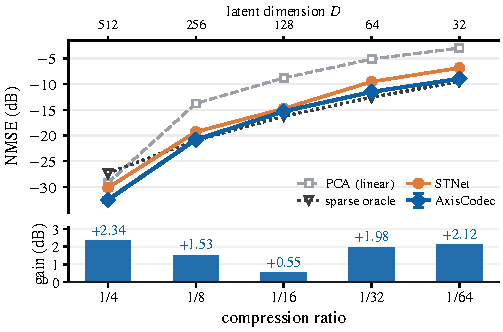
\includegraphics[width=\columnwidth]{fig4_rd.pdf}
\caption{Rate--distortion on COST2100 indoor. PCA and the free-support sparse
oracle are evaluated at the stated budget. AxisCodec beats the 512-dimensional PCA
subspace by 3.3~dB at CR~$1/4$ and STNet at every ratio; blue numbers below the
axis are gains over STNet, and error bars are seed standard deviations at
CR~$1/4$.}
\label{fig:rd}
\end{figure}

\begin{figure*}[!t]
\centering
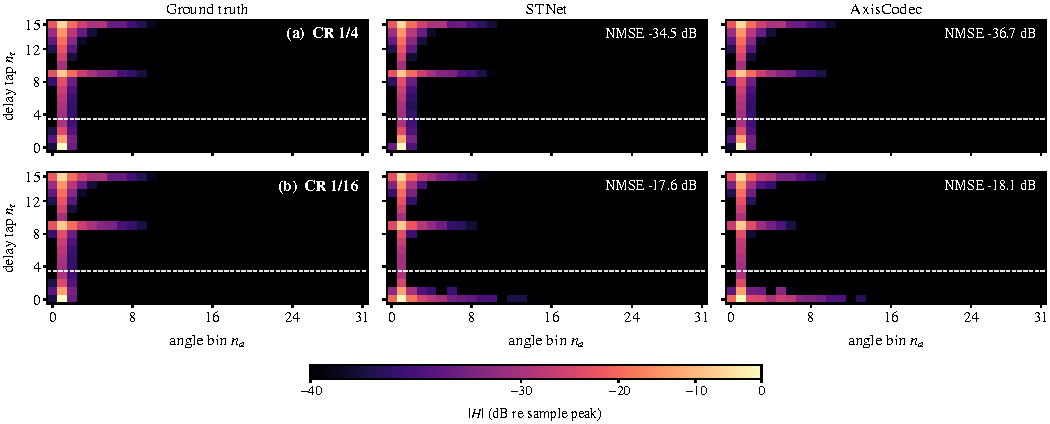
\includegraphics[width=\textwidth]{fig5_qual.pdf}
\caption{Same test channel compressed at CR~$1/4$ (a) and CR~$1/16$ (b). The
sample is the median per-sample NMSE of AxisCodec at CR~$1/4$, so neither model is
favoured. Colour is $|H|$ in dB relative to the sample peak; taps 16--31 carry
0.9\% of the energy and are omitted; the dashed line marks the head/tail split.
Numbers are per-sample NMSE.}
\label{fig:qual}
\end{figure*}

\subsection{Qualitative behaviour}
Fig.~\ref{fig:qual} shows the same channel at two rates. At CR~$1/4$ the head looks
identical to the ground truth for both models, yet the per-tap relative error over
taps 2--5 is $1.5$--$2.3\%$ for STNet and $0.16$--$0.25\%$ for AxisCodec---an order
of magnitude---which sharpens the tap-3/tap-4 ridge in the third column. At
CR~$1/16$ both models blur that ridge and the per-sample gap falls to $0.4$~dB,
matching the matrix-level $0.55$~dB. The gain is thus a systematic reduction of the
mid-tap error that dominates the residual, not a global sharpening.

\subsection{Ablations}
Table~\ref{tab:abl} isolates the three design choices at 300 epochs, where a full
sweep is affordable. Replacing the metric-aligned objective by MSE costs
$1.50$~dB; removing the linear base $0.44$~dB; replacing the circulant angle mixer
by a dense $32\times32$ map $0.25$~dB while raising FLOPs by $1.4\times$. The
objective remains the largest contributor at convergence ($3.0$~dB at 1000
epochs, against $1.50$~dB at 300), while the prior is the cheapest choice and the
only one that reduces compute.

A per-sample breakdown shows the gain is spread over the power distribution:
$1.4$--$1.6$~dB in every quartile at 300 epochs, $2.6$--$3.3$~dB at 1000, and
largest for the weakest channels, which the per-user normalisation weights most.

\begin{table}[!t]
\centering
\caption{Ablations at CR~$1/4$, 300 epochs, seed 0 (NMSE in dB). Positive $\Delta$
is worse.}
\label{tab:abl}
\small
\begin{tabular}{@{}lccc@{}}
\toprule
Variant & NMSE & $\Delta$ & FLOPs \\
\midrule
Full model & $\mathbf{-28.98}$ & --- & 0.022\,G\\
MSE objective & $-27.49$ & $+1.50$ & 0.022\,G\\
No linear base & $-28.55$ & $+0.44$ & 0.022\,G\\
Dense angle mixer & $-28.74$ & $+0.25$ & 0.030\,G\\
\bottomrule
\end{tabular}
\end{table}

\subsection{Error analysis across compression}
The head/tail split explains the non-monotone gain pattern
(Table~\ref{tab:headtail}). At CR~$1/4$ the head relative error is
$3.0\times10^{-5}$ for AxisCodec and $3.7\times10^{-4}$ for STNet; at CR~$1/16$
both degrade to $\sim2\times10^{-2}$, because 128 real numbers cannot pin down a
field that carries 92\% of its energy in four taps; at CR~$1/64$ they reach
$1.0\times10^{-1}$ and $1.8\times10^{-1}$. Wherever the head is still
representable, our linear base converts that into a large gain; where it is not,
the gain narrows. At CR~$1/64$ the model nevertheless improves both head and tail,
and $\rho$ gains $0.043$---a larger relative improvement than NMSE, which matters
for downstream beamforming.

\begin{table}[!t]
\centering
\caption{Head (taps 0--3) and tail (taps 4--31) relative error
$\|\Hh-\Hb\|^2/\|\Hb-0.5\|^2$ per region, averaged over the test set.}
\label{tab:headtail}
\footnotesize
\begin{tabular}{@{}lcccc@{}}
\toprule
& \multicolumn{2}{c}{STNet} & \multicolumn{2}{c}{AxisCodec}\\
\cmidrule(lr){2-3}\cmidrule(lr){4-5}
CR & head & tail & head & tail \\
\midrule
1/4 & $3.7{\times}10^{-4}$ & $9.4{\times}10^{-3}$ & $3.0{\times}10^{-5}$ & $7.6{\times}10^{-3}$\\
1/16 & $2.2{\times}10^{-2}$ & $2.6{\times}10^{-1}$ & $1.7{\times}10^{-2}$ & $2.4{\times}10^{-1}$\\
1/64 & $1.8{\times}10^{-1}$ & $7.7{\times}10^{-1}$ & $1.0{\times}10^{-1}$ & $7.5{\times}10^{-1}$\\
\bottomrule
\end{tabular}
\end{table}

\subsection{Complexity and stability}
Table~\ref{tab:cx} lists parameters and FLOPs. AxisCodec matches STNet in
parameters and costs $1.6\times$ its FLOPs, the price of full-resolution mixing.
A narrower variant (4 channels) runs at 0.011~GFLOPs, below STNet, and has not been
validated at 1000 epochs.

\begin{table}[!t]
\centering
\caption{Complexity at CR~$1/4$ (single-sample forward pass).}
\label{tab:cx}
\small
\begin{tabular}{@{}lccc@{}}
\toprule
Model & Parameters & Effective & FLOPs \\
\midrule
CsiNet & 2.10\,M & 2.10\,M & 0.011\,G\\
CLNet & 2.10\,M & 2.10\,M & 0.008\,G\\
STNet & 3.18\,M & 2.13\,M & 0.014\,G\\
AxisCodec & 2.13\,M & 2.13\,M & 0.022\,G\\
\bottomrule
\end{tabular}
\end{table}

Fig.~\ref{fig:train} shows why the schedule matters. With its published constant
learning rate, STNet reaches its operating point near epoch 450 and then oscillates
within 3.7~dB for the rest of training; AxisCodec, annealed with a cosine schedule,
passes through the same region later and keeps improving to the end. Its validation
NMSE at epoch 300 is 2.0~dB worse than STNet's and 2.3~dB better at epoch 1000, so
a 300-epoch comparison undersells the architecture---which is why every entry of
Table~\ref{tab:main} uses 1000 epochs.

\begin{figure}[!t]
\centering
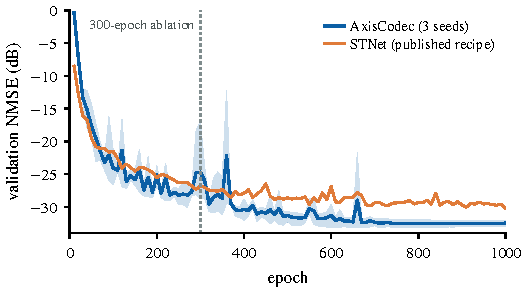
\includegraphics[width=\columnwidth]{fig6_train.pdf}
\caption{Validation NMSE against epoch. The band is the range over three seeds of
AxisCodec; STNet follows its published constant-learning-rate recipe. The dashed
line marks the 300-epoch budget used for ablations.}
\label{fig:train}
\end{figure}

Training is stable once the learning rate anneals: over the last 300 epochs the
test NMSE varies with a standard deviation of $0.07$--$0.10$~dB across seeds
($0.03$~dB over the last 100), so the $2.34$~dB margin is more than twenty times
the noise of the final phase.
Between epochs 90 and 660 the model occasionally collapses by 8--18~dB for a
single validation evaluation and recovers within twenty epochs
(Fig.~\ref{fig:train}); the training loss stays flat through these events, so they
are generalisation transients rather than divergence, and validation-based
selection absorbs them.

\section{Discussion}
\textbf{Why the geometric prior is worth only 0.25~dB.} A circulant mixer is a
32-parameter constraint on a 1024-parameter operator: it fixes the wrap-around at
bins 0 and 31 and forbids a dense map from treating them as distant. Angular
profiles in this data are smooth enough that a dense mixer learns nearly the same
operator from 100k samples, so the constraint buys a $32\times$ smaller operator and
$1.4\times$ fewer FLOPs rather than accuracy. The priors that did move NMSE---the
metric-aligned objective and the linear/residual split---act on \emph{how bits are
distributed}, which is why they are worth 1.50 and 0.44~dB.

\textbf{Why long training matters.} A 300-epoch run of the same recipe is
3.5~dB behind the 1000-epoch one, and the gain is concentrated in the tail: its relative error
falls from $1.7\times10^{-2}$ to $7.6\times10^{-3}$. Tail coefficients are small
and their gradients weak, so they need a long anneal; any conclusion drawn at 300
epochs underestimates this architecture.

\textbf{Practical rules.} Two lessons transfer beyond this benchmark. First, match
the training objective to the reported metric: here that is worth 1.5--3~dB,
more than any architectural change we tried. Second, spend parameters on the geometry of
the representation rather than on a channel model the data does not obey. For a
uniform planar array the angle axis becomes a two-torus, so one circulant mixer
becomes two at $2N$ parameters per channel, while the delay path is unchanged. What
must be re-checked, not assumed, is the diagnostic: fit the parametric family at a
matched rate against a free sparse code before adopting a path-based design.

\textbf{Limitations.} All results are on COST2100. Its diffuse angular--delay
energy is what invalidates parametric models here; on a more specular dataset, such
as a CDL-C-like model with strong line-of-sight, path-based coding could become
competitive again; our oracle procedure is the way to check. Multi-seed
evidence covers CR~$1/4$; the other ratios are single-seed. The model costs
$1.6\times$ STNet's FLOPs. The latent is assumed noiseless, as in the baselines;
how the geometry prior interacts with a quantiser is left open. Finally, the
transients described above indicate a rougher optimisation landscape than STNet's,
which is a clear target for future work.

\textbf{Reproducibility.} Every configuration is a YAML file fixing the model,
optimiser, schedule and seed; each run writes a \texttt{metrics.json} with the
commit, the selected checkpoint and its re-evaluated NMSE and $\rho$. Baselines use
the repository's own implementations; the oracle fits, scripts and checkpoints
behind every number and figure are included.
A 1000-epoch run takes 3.9~h on one RTX~5090.

\section{Conclusion}
Compact parametric channel models do not describe COST2100: rate-matched oracle
fits of Dirichlet atoms, harmonic subspaces and Gaussian blobs all lose by wide
margins to a free sparse code. What does describe it is the geometry of the
representation and the distribution of the residual. Encoding that geometry as
circulant angle mixing and dense delay mixing, splitting the decoder into a linear
base and a nonlinear residual, and training on the reported per-user NMSE yields
$-32.52\pm0.55$~dB at CR~$1/4$ against $-30.17$~dB for STNet, with equal
effective parameters and a $1.6\times$ FLOP budget.

\begin{thebibliography}{24}
\bibitem{wen2018} C.-K. Wen, W.-T. Shih, and S. Jin, ``Deep learning for massive
MIMO CSI feedback,'' \emph{IEEE Wireless Commun. Lett.}, vol.~7, no.~5,
pp.~748--751, 2018.
\bibitem{wang2019} T. Wang, C.-K. Wen, S. Jin, and G. Y. Li, ``Deep learning-based
CSI feedback approach for time-varying massive MIMO channels,'' \emph{IEEE
Wireless Commun. Lett.}, vol.~8, no.~2, pp.~416--419, 2019.
\bibitem{lu2020} Z. Lu, J. Wang, and J. Song, ``Multi-resolution CSI feedback with
deep learning in massive MIMO system,'' in \emph{Proc. IEEE ICC}, 2020, pp.~1--6.
\bibitem{ji2021} S. Ji and M. Li, ``CLNet: Complex input lightweight neural network
designed for massive MIMO CSI feedback,'' \emph{IEEE Wireless Commun. Lett.},
vol.~10, no.~10, pp.~2318--2322, 2021.
\bibitem{cvl2022} H. Li \emph{et al.}, ``CVLNet: A complex-valued lightweight
network for CSI feedback,'' \emph{IEEE Wireless Commun. Lett.}, vol.~11, no.~5,
pp.~1092--1096, 2022.
\bibitem{trabelsi2018} C. Trabelsi \emph{et al.}, ``Deep complex networks,'' in
\emph{Proc. ICLR}, 2018.
\bibitem{cui2022} Y. Cui, A. Guo, and C. Song, ``TransNet: Full attention network
for CSI feedback in FDD massive MIMO system,'' \emph{IEEE Wireless Commun. Lett.},
vol.~11, no.~5, pp.~903--907, May 2022.
\bibitem{mourya2023} S. Mourya, S. Amuru, and K. K. Kuchi, ``A spatially separable
attention mechanism for massive MIMO CSI feedback,'' \emph{IEEE Wireless Commun.
Lett.}, vol.~12, no.~1, pp.~40--44, 2023.
\bibitem{lou2025} K. Lou, H. Ji, and X. Wu, ``Attention-infused autoencoder for
massive MIMO CSI compression,'' in \emph{Proc. IEEE Wireless Commun. Netw. Conf.
(WCNC)}, 2025, pp.~1--6.
\bibitem{ansarifard2025} M. Ansarifard \emph{et al.}, ``CSI compression beyond
latents: End-to-end hybrid attention-CNN networks with entropy regularization,''
arXiv:2509.08776, 2025.
\bibitem{cai2019} Q. Cai, C. Dong, and K. Niu, ``Attention model for massive MIMO
CSI compression feedback and recovery,'' in \emph{Proc. IEEE Wireless Commun. Netw.
Conf. (WCNC)}, 2019, pp.~1--5.
\bibitem{saldr2021} X. Song \emph{et al.}, ``SALDR: Joint self-attention learning
and dense refine for massive MIMO CSI feedback with multiple compression ratio,''
\emph{IEEE Wireless Commun. Lett.}, vol.~10, no.~9, pp.~1899--1903, Sep. 2021.
\bibitem{guo2022model} J. Guo \emph{et al.}, ``CSI feedback with model-driven deep
learning of massive MIMO systems,'' \emph{IEEE Commun. Lett.}, vol.~26, no.~3,
pp.~547--551, 2022.
\bibitem{liu2022markov} Z. Liu, M. del Rosario, and Z. Ding, ``A Markovian
model-driven deep learning framework for massive MIMO CSI feedback,'' \emph{IEEE
Trans. Wireless Commun.}, vol.~21, no.~2, pp.~1214--1228, Feb. 2022.
\bibitem{ma2023typeii} K. Ma \emph{et al.}, ``Deep learning empowered Type-II
codebook: New paradigm for enhancing CSI feedback,'' arXiv:2305.08081, 2023.
\bibitem{qin2025} Z. Qin and H. Yin, ``A review of codebooks for CSI feedback in 5G
new radio and beyond,'' \emph{China Commun.}, vol.~22, no.~2, pp.~112--127, 2025.
\bibitem{liu2021ev} W. Liu \emph{et al.}, ``EVCsiNet: Eigenvector-based CSI feedback
under 3GPP link-level channels,'' \emph{IEEE Wireless Commun. Lett.}, vol.~10,
no.~12, pp.~2688--2692, 2021.
\bibitem{kim2025} H. Kim \emph{et al.}, ``Generative diffusion model-based
compression of MIMO CSI,'' in \emph{Proc. IEEE Int. Conf. Commun. (ICC)}, 2025,
pp.~1--6.
\bibitem{guo2025onesided} Y. Guo \emph{et al.}, ``Deep learning for CSI feedback:
One-sided model and joint multi-module learning perspectives,'' \emph{IEEE Commun.
Mag.}, vol.~63, no.~7, pp.~90--97, 2025.
\bibitem{liu2012cost} L. Liu \emph{et al.}, ``The COST 2100 MIMO channel model,''
\emph{IEEE Wireless Commun.}, vol.~19, no.~6, pp.~92--99, 2012.
\bibitem{3gpp38843} 3GPP, ``Study on artificial intelligence (AI)/machine learning
(ML) for NR air interface,'' TR 38.843 V18.0.0, Dec. 2023.
\bibitem{3gpp38214} 3GPP, ``NR; physical layer procedures for data,'' TS 38.214
(Rel-18).
\end{thebibliography}

\balance
\end{document}
